%This chapter/section is about the work on ``dc-smearing in GPP''
%Created by kp on Sep 17, 2011

%\hspace{0.5cm}
% \newline \newline
%\newline  %double \newline gives underfull warnings

\begin{comment}
This is here just to remind me about this way of making comments
And, also to add some more reminders to myself.
1) change the figure size parameters to fit to the page if possible. 2) if related, put two or more figures side by side to save space as well as to make the organization better (otherwise, the compiler may put figures randomly and thus losing the sense of order/continuity)

It is assumed that the efficiency depends on the number of photoelectrons (the corresponding variable in the data ntuple is ``nphe''), which in turn is determined by the hit location on the Cerenkov PMT-projected plane (defined by the projected 
\th and \ph) as well as the angle with which the particle hit the plane. \ref{fig:genEvnts3}
\end{comment}

%%%%%%%%%%%%%%%%%%%
%   Note: The following section disabled because it is also in introChp4Sim.tex which includes this file with \input{filename}
%%%%%%%%%%%%%%%%%%%
%\section{GSIM POST PROCESSOR (GPP)}  
A lot of known, unknown, quantified, and unquantified factors such as temperature, alignment, dead channels, electronic malfunction etc affect the performance of the CLAS detector. But, GSIM does not include all these effects and, hence, the efficiency of the detector is always less than what the simulation provides us. To make the simulation more realistic by taking into account some of those effects, another CLAS software called GSIM Post Processor (GPP) is used to process the GSIM output. The GPP can change the DC, SC, CC and EC signals produced in the simulation\footnote{The DC signals can be changed by (a) accounting for the dead wires according to the calibration database, (b) shifting the DOCA mean value, and (3) smearing the hit signals according to the resolution determined by the calibration database or according to the command line input. Likewise, SC signals can be changed with a parameter input for smearing the time resolution. And, for %the CC and %SEK: We didn't include the CC in sim.
EC signals, the GPP can use the hardware thresholds \cite{jxZhang_th}.}.

As the experimental conditions and detector configurations can change from one experiment to another, in order to run the GPP, we must have our own experiment specific calibration constants and parameters such as the run number (R), the DC smearing scale values for regions 1, 2 and 3 (a, b, c) and the SC smearing scale value (f). Even for a given experiment, these constants and parameters are determined to be different for different data sets (corresponding to a given beam energy, for example). The value for R can be any run number belonging to a specific data set. This number is used to identify the entry of the calibration constants in the database that corresponds to the given data set.  In order to simplify the job, we decided to use the timing resolutions determined by the calibration database assuming that they are good enough and need only to determine new values for the DC smearing. %(the reason to do this is that with the default (calibration database) resolution, the energy resolution in the data and the simulation seemed to differ significantly (as will be evident below when we compare the widths of the simulation & real data elastic peaks) 
To further simplify the job, we assumed that the three DC Regions had identical resolutions, so the DC smear parameters a, b, and c would have the same values, and the common DC-smear value is what is determined from the procedure described below.



%\subsection{\href{http://www.jlab.org/Hall-B/secure/eg4/adhikari/Analysis/SimStuffs/moniDcSmear.html}{Determining Dc-smear scales for GPP} to have the energy resolution of simulation comparable with that of the CLAS}
In order to determine the DC-smear, we generated a statistically significant number (about half million) of elastic-electron events distributed according to the elastic cross section and then ran them through GSIM, GPP and RECSIS. The pure proton target events, turning off the radiative effects are generated using the existing %Genova inherited 
STEG event generator. %As an example, the 2.3 GeV events looked like as shown in fig(\ref{fig:genEvnts3}) when histogrammed in the quantity $\Delta$E.

%(/w/hallb/claseg4/adhikari/GSIM_RECSIS/mod_osip_bost/mod_osip_bostVadim11_64tNH3). I modified the two files sgm_model.f & cor_peak_proton.f 
%which are kept for backup in the same directory where eps files are. In addition, the routines of bost.f were replaced with the latest 
%(/w/hallb/claseg4/adhikari/GSIM_RECSIS/bost09.f, soft linked by the old name bost.f), both generate_map and work directories use all these three files
% See my comments on cor_peak_proton.f at the very bottom of this file
\begin{comment} %Disabling this one to replace it with a figure that his a caption on the side rather than at the bottom.
\begin{figure}[h] %ht, htpb (p - float, b = bottom, h=? t = top)
  \leavevmode 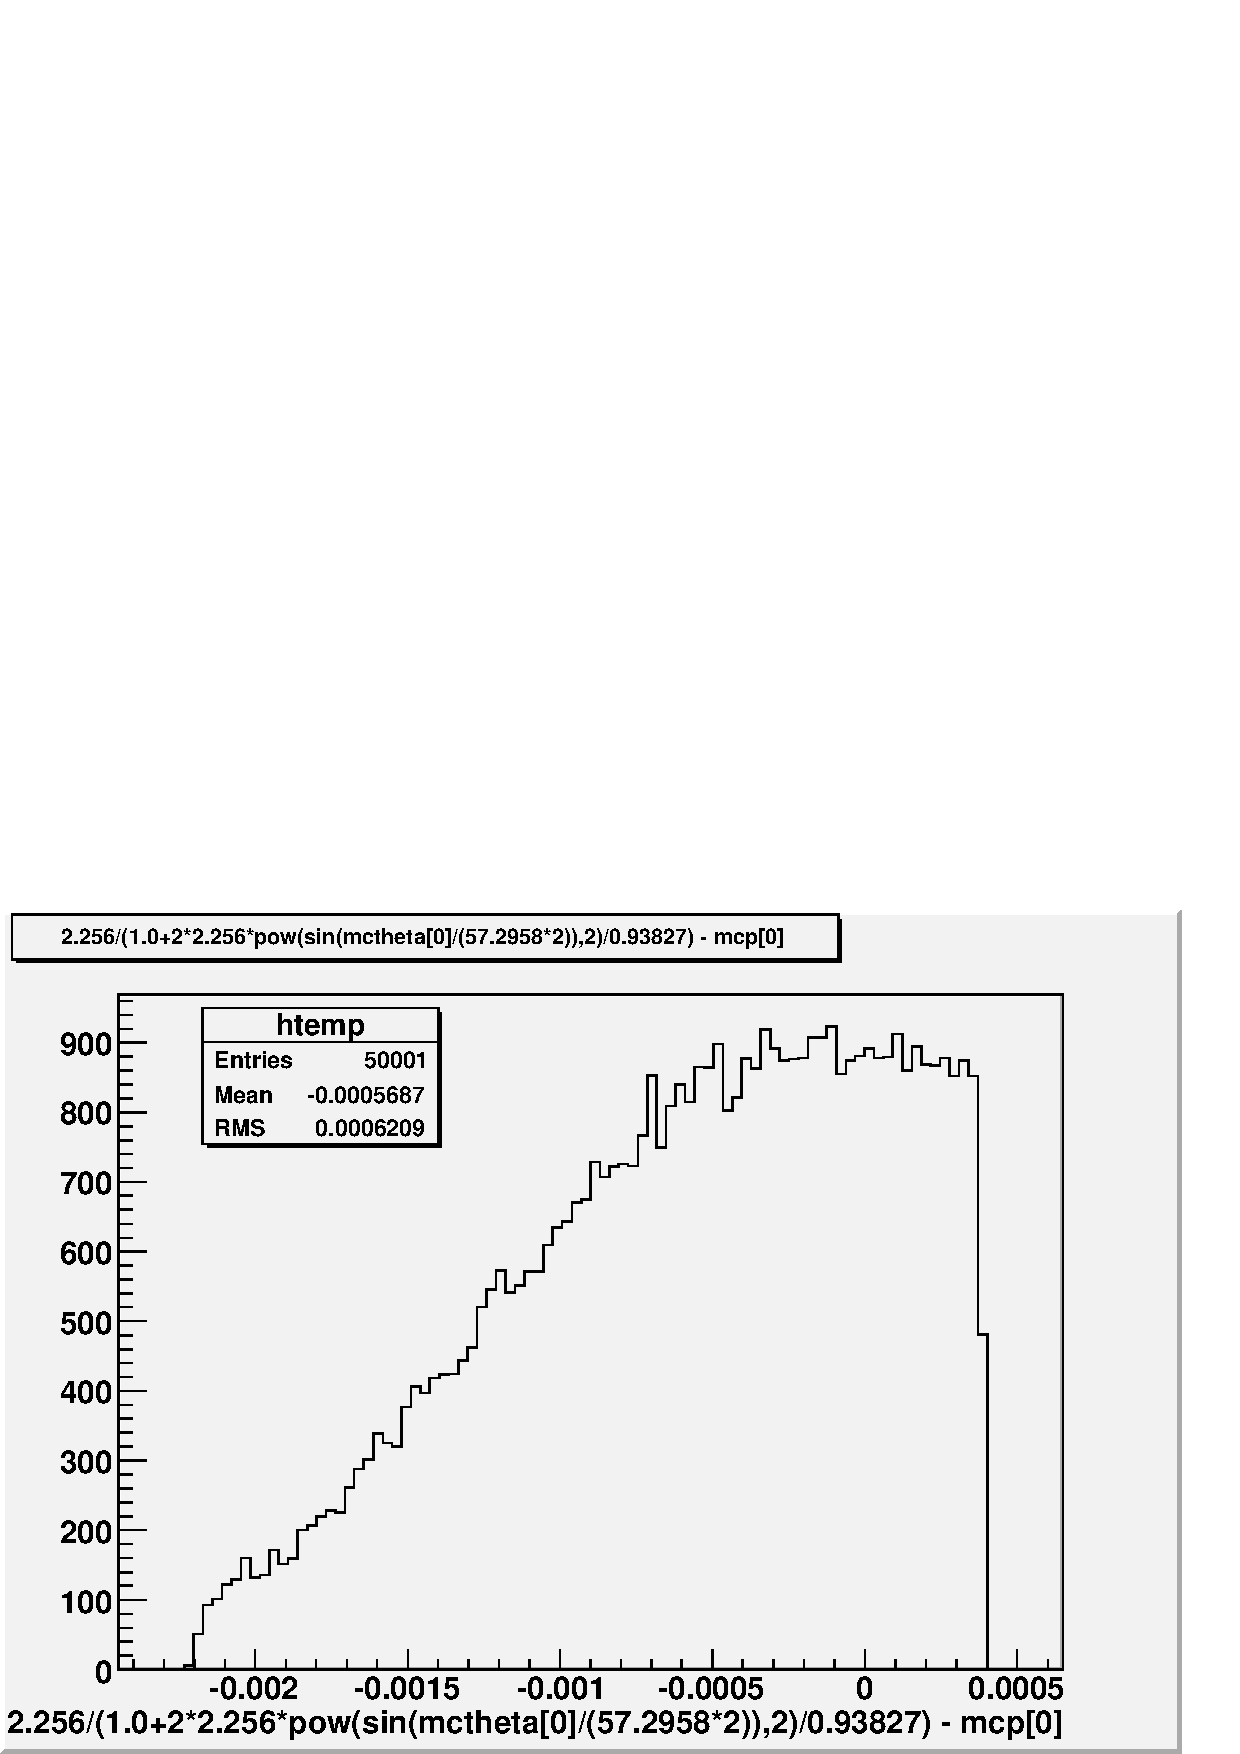
\includegraphics[width=0.6\textwidth]{figuresEG4/DcSmear/genEvntsElastOnlyEb3.png} 
  \caption[$\Delta$E of generated elastic events]{$\Delta$E of 2.3 GeV generated elastic-only proton-target events (no internal radiative effects).}
  \label{fig:genEvnts3}
\end{figure}



\begin{SCfigure} %http://en.wikibooks.org/wiki/LaTeX/Floats,_Figures_and_Captions (needs packages \usepackage[pdftex]{graphicx} & \usepackage{sidecap})
  \centering
  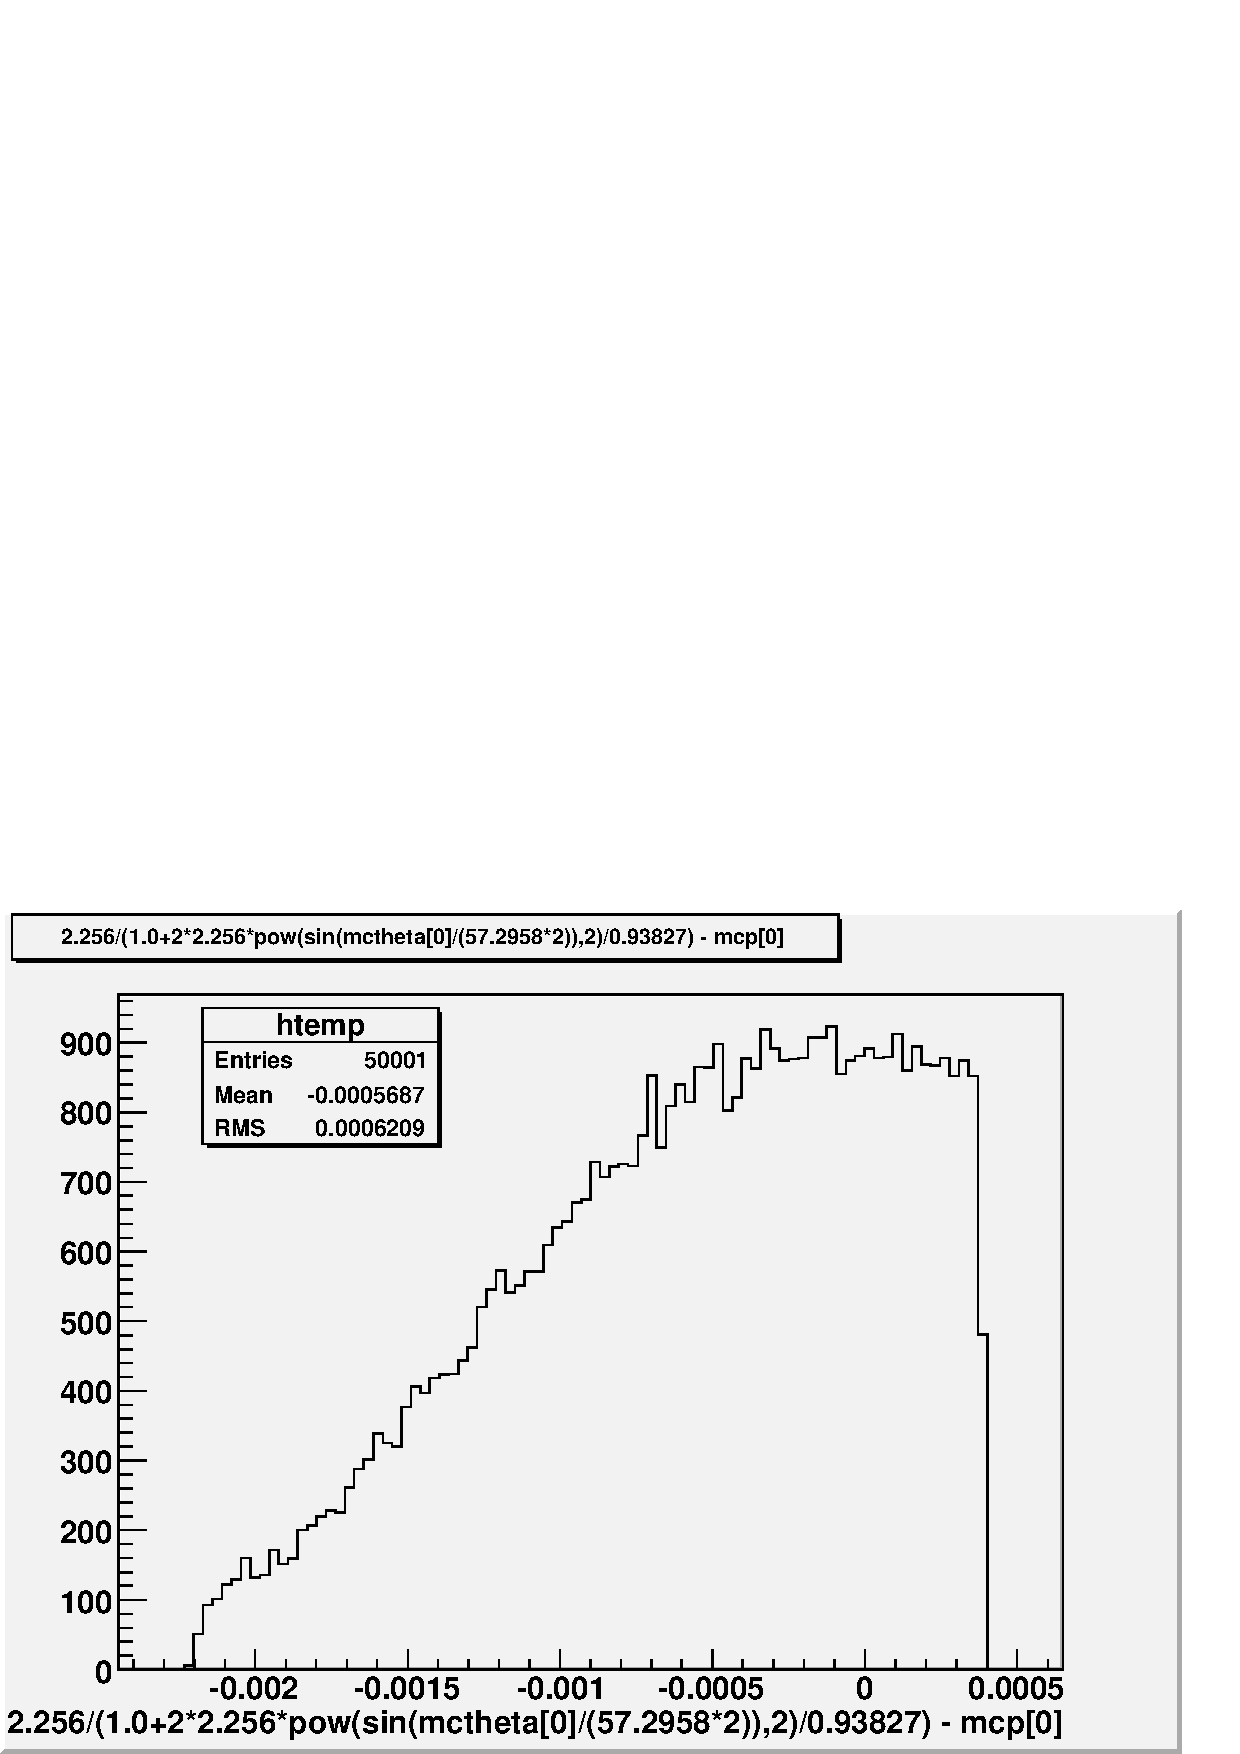
\includegraphics[width=0.7\textwidth]{figuresEG4/DcSmear/genEvntsElastOnlyEb3.png}
  \caption[$\Delta$E of generated elastic events]{$\Delta$E of 2.3 GeV generated elastic-only proton-target events (no internal radiative effects).}
  \label{fig:genEvnts3}
\end{SCfigure}

 \end{comment}

%\subsection{Finding the variation of the width of the simulated elastic peak as a function of DC-smear scale for GPP.}
The simulated elastic events are then fed into GSIM, GPP and RECSIS, with GSIM and RECSIS used in the same configuration as when processing the CLAS data 
during the ``pass-1'' phase, and GPP run with different values of DC-smear scales as inputs. The reconstructed data coming out of RECSIS corresponding to 
a given value of DC-smear is then histogrammed in $\Delta$E again and fitted to a Gaussian to get its $\sigma$ (characterizing width) and mean (characterizing position). As we can see in figures \ref{fig:dcSm1.3} and \ref{fig:dcSm2.9}, %fig(\ref{fig:dcSmEff}), %This didn't give proper number
the width of the elastic peak increases with the DC-smear but the position stays more or less the same as expected. In fact, when the two are plotted 
against DC-smear (as in figures \ref{fig:SigmaVsm} and \ref{fig:MeanVsm}) %(as in fig (\ref{fig:ParsVsm})), %This didn't give proper number 
the width shows a linear dependance.






% idea source: http://texblog.wordpress.com/2007/08/28/placing-figurestables-side-by-side-subfigure/ :Placing figures/tables side-by-side (\subfigure)
% Can include any number of figures/tables, not just two.
\begin{figure}[H]
\centering
\subfigure[Dc-smear]{
\includegraphics[scale=0.32]{figuresEG4/DcSmear/dE_ThAllEb3_DcSmear1p3}%.png}
\label{fig:dcSm1.3}
}
\subfigure[Dc-smear]{
\includegraphics[scale=0.32]{figuresEG4/DcSmear/dE_ThAllEb3_DcSmear2p9}%.png}
\label{fig:dcSm2.9}
}
\label{fig:dcSmEff} %Effect of Dc-smear
%\caption[Optional caption for list of figures]{Caption of subfigures \subref{fig:subfig1}, \subref{fig:subfig2} and \subref{fig:subfig3}}
\caption[$\Delta$E of reconstructed simulated events]{$\Delta$E of 2.3 GeV simulated elastic-only proton-target events passing through GSIM, GPP (with two different Dc-smear scales of 1.3 (a) and 2.9 (b)), and RECSIS.}
\end{figure}




\begin{figure}[H]
\centering
\subfigure[$\sigma$ vs DC-smear]{
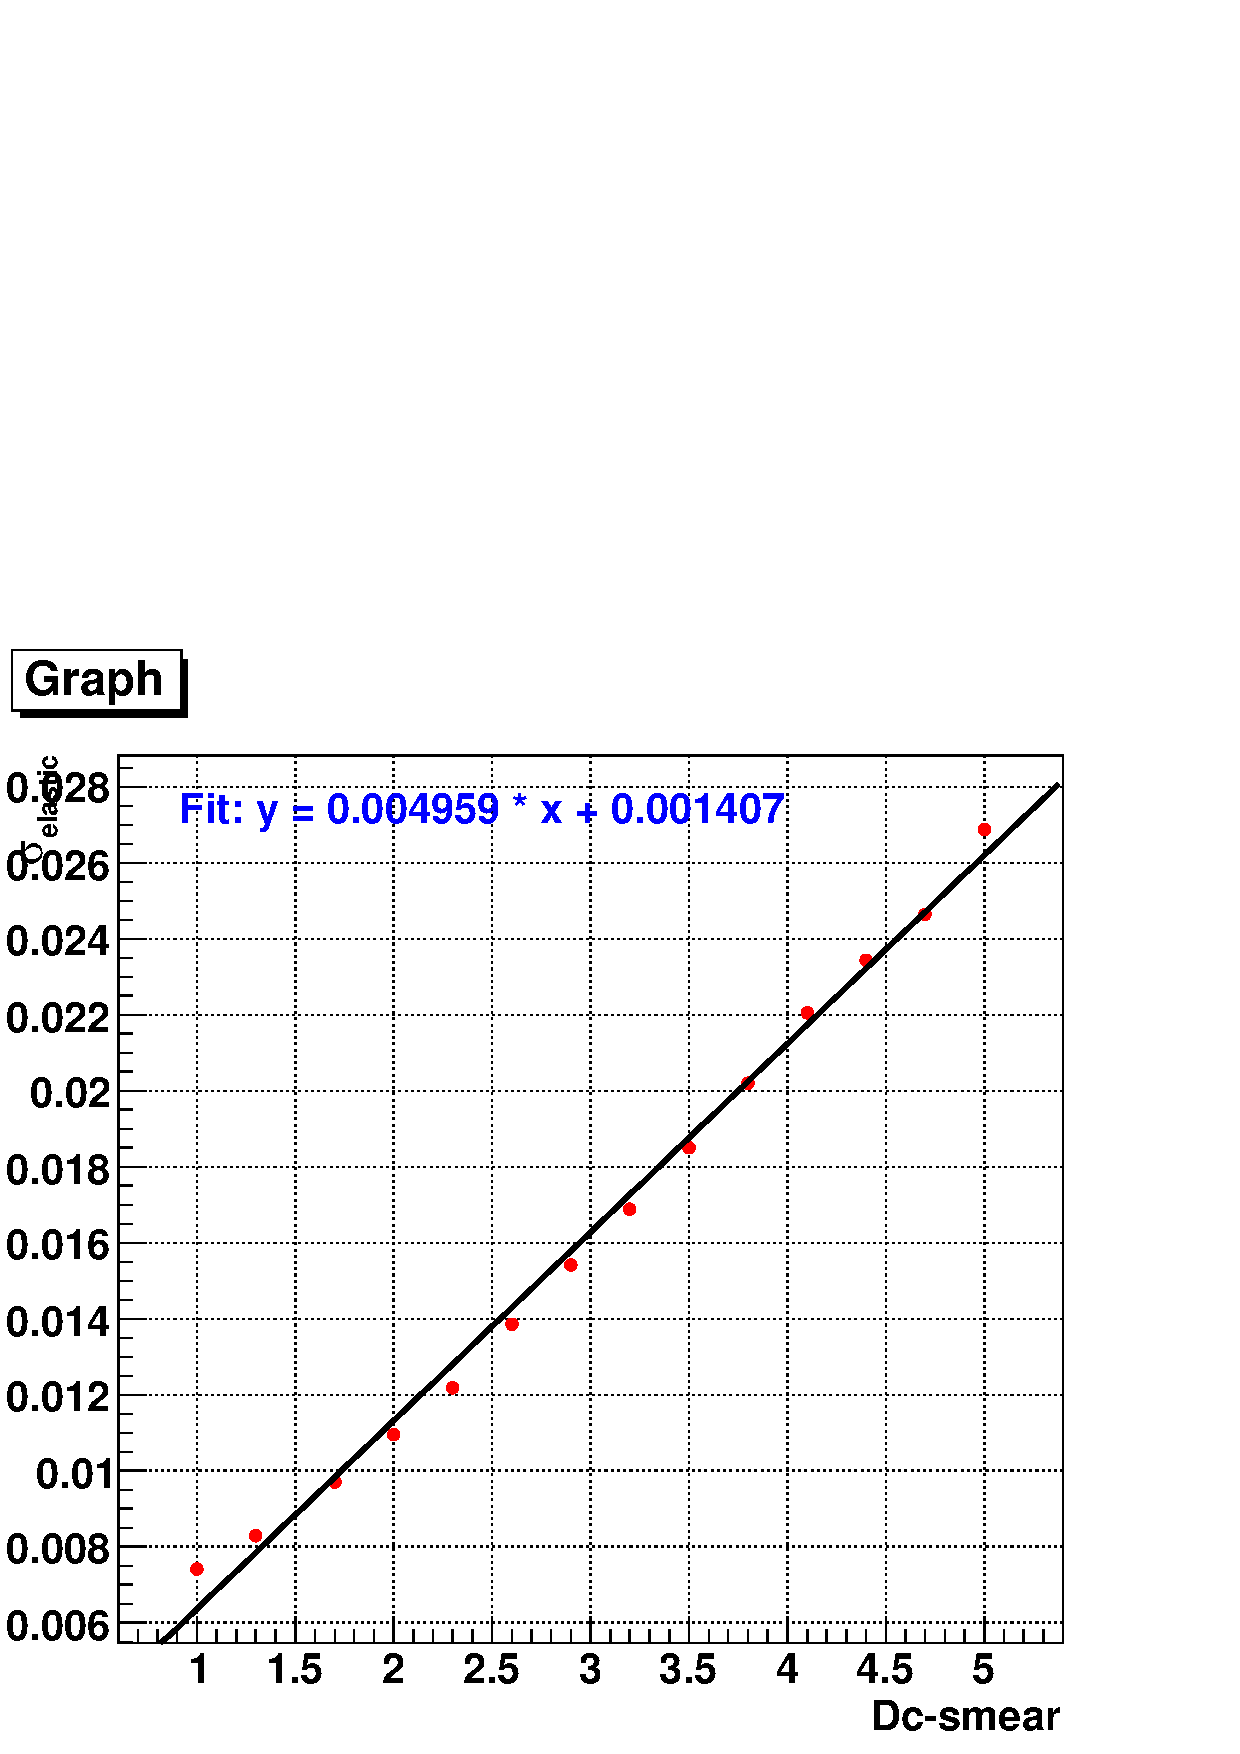
\includegraphics[scale=0.32]{figuresEG4/DcSmear/grSigmaVsDcSmear_Eb3.png}
\label{fig:SigmaVsm}
}
\subfigure[Mean vs DC-smear]{
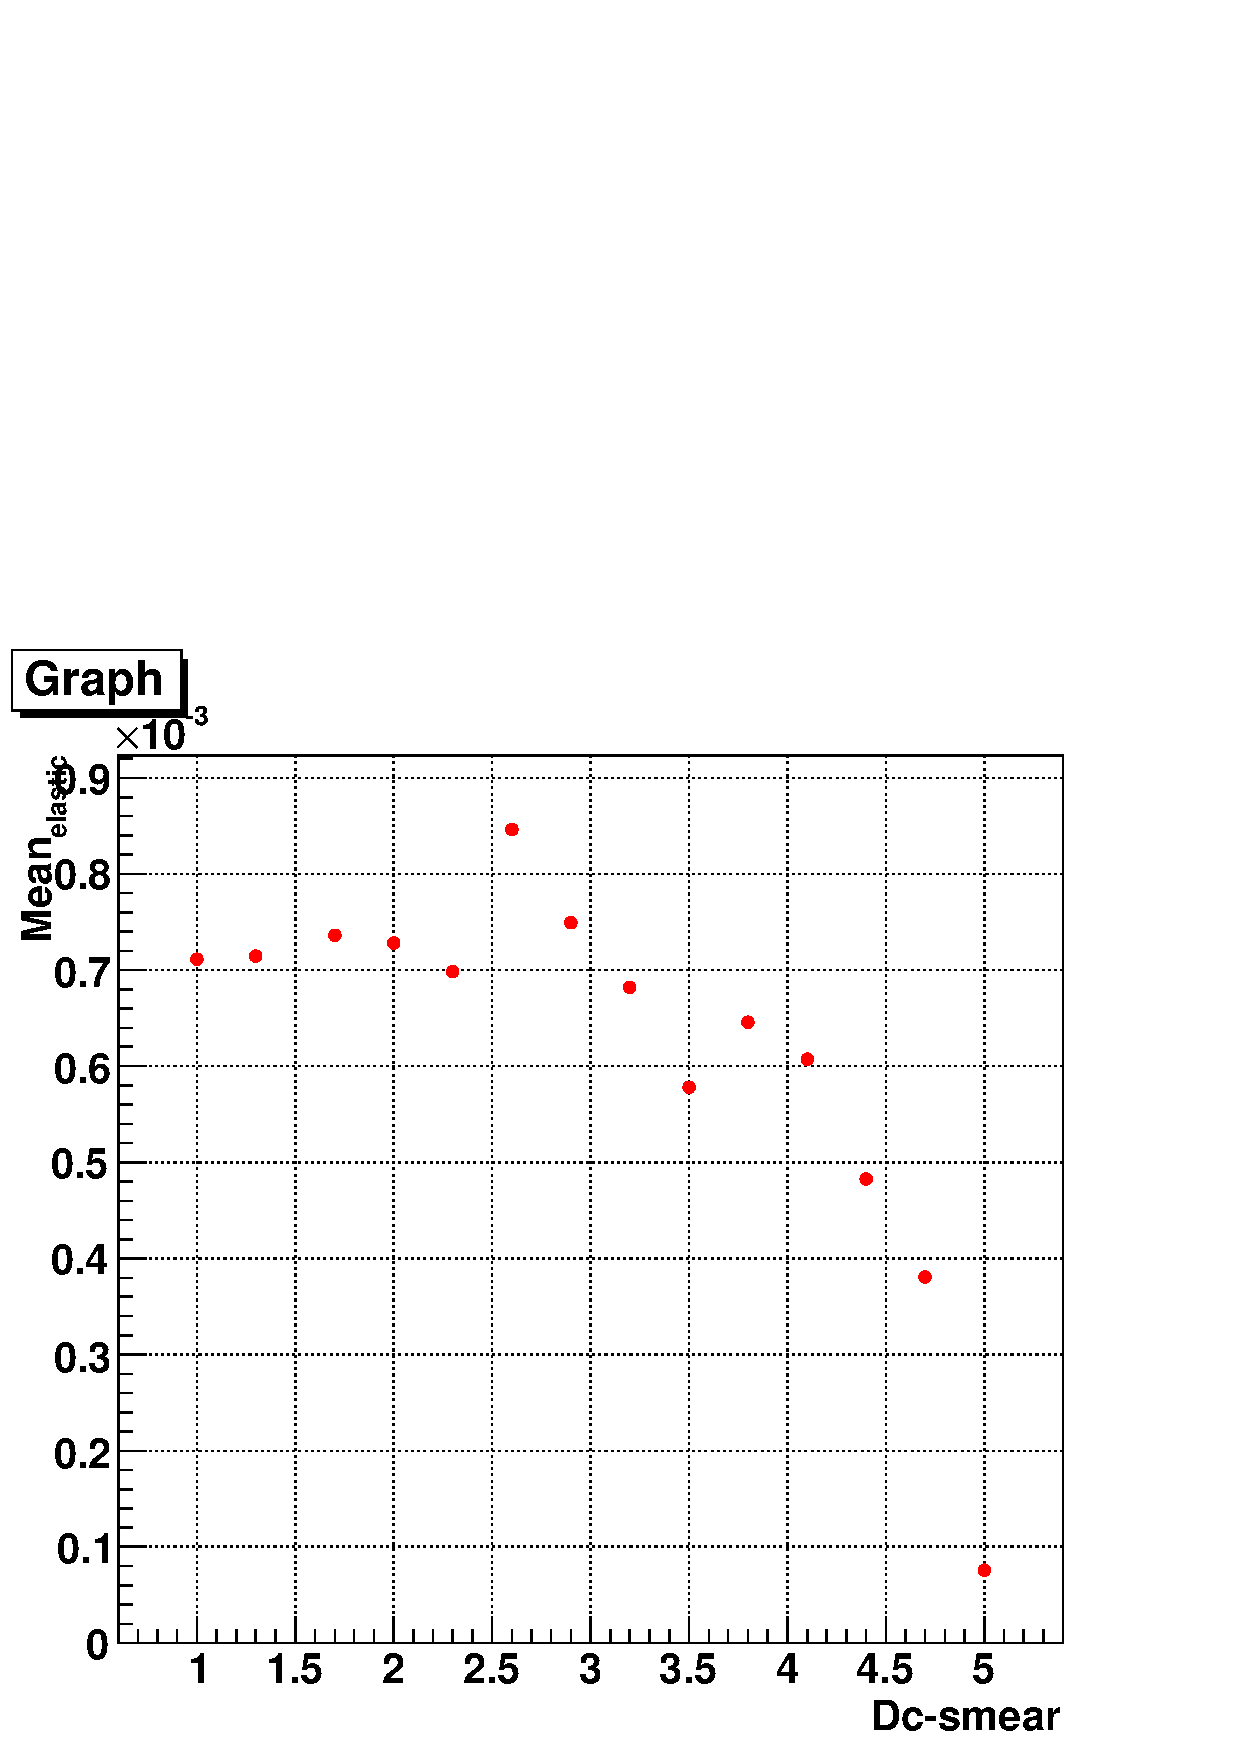
\includegraphics[scale=0.32]{figuresEG4/DcSmear/grMeanVsDcSmear_Eb3.png}
\label{fig:MeanVsm}
}
\label{fig:ParsVsm} %Effect of Dc-smear
%\caption[Optional caption for list of figures]{Caption of subfigures \subref{fig:subfig1}, \subref{fig:subfig2} and \subref{fig:subfig3}}
\caption[DC-smearing effects on elastic peak]{Graphs showing the dependence of width and position (obtained from the Gaussian fits as shown in the fig (\ref{fig:dcSmEff}) of the elastic peaks on the DC-smear applied to GPP.}
\end{figure}


%\subsection{Finding the width of the real CLAS data elastic peak.}
With the knowledge of the DC-smear dependence of energy resolution (Fig. \ref{fig:SigmaVsm}), we can look at the resolution in the real data such as the one estimated in Fig. \ref{sec6dEall}, 
and then determine the right value of DC-smear which would make the resolution in the simulation comparable with that in the real data. By repeating this process of comparing the experimental and simulated resolutions for each of the beam energies, the values of the DC-smear parameters for the GPP were deterimined as listed in Table. \ref{tab:dcSmears} below.


%\FloatBarrier  
% \FloatBarrier %http://tex.stackexchange.com/questions/9485/how-to-fix-table-position
%\begin{center}
\begin{table}[H]%[h] %[h!b!p!]
\centering
    \caption{DC-smearing scales determined for different beam energies.}
    \label{tab:dcSmears}
    \begin{tabular}{ | l | l | l | l | l | l |}
    \hline
    $E_{beam}$ (GeV) & 1.054  & 1.339 & 1.989 & 2.256 & 2.999 \\ \hline
    DC-smear         & 2.6    & 2.0   & 2.0   & 2.0   & 1.7 \\  \hline
    \end{tabular}
%    \caption{DC-smearing scales determined for different beam energies.}
%    \label{tab:dcSmears}
\end{table}
%\end{center}




\begin{comment} %==================My comments on the generated events==========Comments begin=== Sep 19, 2011
%The events were generated by using the Genova inherited mod_osip_bost (aka STEG) generator 
      subroutine smrad_proton(Es,theta,Ep,sig_el,sig_tot,sel,smin)
      common/material/TG
      sn2=(sin(theta/2.0))**2     Q2=4.0*Es*Ep*sn2       nu=Es-Ep
c-----input values
      Mp=0.93827        Z=1      A=1     E3=Es/(1.0+Es*(1.0-cos(theta))/Mp)
c-----elastic peak width==resolution
      dWp=0.001       delta_E=(dWp+dWp**2/(2.0*Mp))/(1.0+2.0*Es/Mp*sn2)/5.
c-----Target thickness
      t=0.0181              ! 0.6 cm NH3
      tiw=0.0079            ! 7.45 mm He
      tfw=0.0079            ! 7.45 mm He

      elra=0.0d+0       innn=0.0d+0       eltail=0.0d+0
c-----cross section
      if(Ep.gt.(E3-2.0*delta_E)) then
      varr=abs(nu-Q2/(2.0*Mp))
      jack=Es/E3
      elcor=elasrad_proton(Es,theta,t,delta_E,Z,A,tiw,tfw)                     ! cole smith program for radiative correction in the elastic region
      elra=sig_elastic_proton(Es,theta,Mp,Z)*elcor*peak_proton(varr,dWp)*jack
      
      innn=0.0d+0
      eltail=0.0d+0
      else
      elra=0.0d+0
      
      streg_tail=straggling_elasic_proton(Z,Mp,t,Es,Ep,theta,delta_E)           !But this is not added to anything so it's inconsequencial
      endif
            
      sel=elra+eltail
      smin=elra+innn+eltail
      return
      END


Comments:
There are two if blocks in the above chunk of the code:
     a) the ``if'' block which covers the elastic region
     b) the  ``else'' block which covers the rest of the region.
The else block has zero contribution to the value returned by the function because we set 'innn' and 'eltail' to zero and 'streg_tail' is not added to 
the sum to be returned.

As we see, the way I did is (being unsure how to turn off the effect of elcor (Cole smith's rad-corr)) leave the target widths t, tiw and tfw as they 
were (i.e. to non-zero values), and also leave the elcor factor alone, so that it would have some modulating effect on the remaining part of the product  
i.e. sig_elastic_proton(Es,theta,Mp,Z)*peak_proton(varr,dWp)*jack. Initially I thought I would give elcor an artificial value of 1.0 and that would 
probably turn off the effect. But, because of lack of confidence in that idea, I abandoned that idea and left it to modulate the elastic peak (may be 
the peak would come out more like a Gaussian, if I had done that). Even with that modulation, the generated events are within 3 MeV range and so the 
modulation would be insignificant. Another thought that came to my mind was that since this factor should have the effect of reducing the events in the 
elastic region to compensate for the radiative tail that we get beyond the elastic region, and since we're not simulating that part, there is no point 
in worrying about that reduction. If if the factor reduced the cross-section, the generator would produce the same number of events by running some extra 
mile to compensate for that reduction. 
\end{comment}  %=======================================Comments end
